% -*- coding: utf-8 -*-
% Линеаризованное ветвление
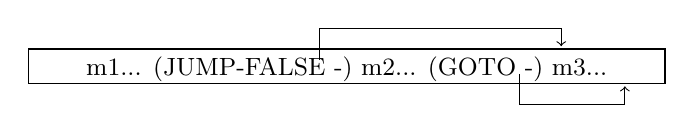
\begin{tikzpicture}
  \tikzstyle{every node}=[font=\small]

  \draw [semithick] (0em, 0em) rectangle (23em, 1.25em);
  \draw (11.5em, 1.33em) node[below]
        {\ic{m1... (JUMP-FALSE -) m2... (GOTO -) m3...}};

  \draw [->] (10.525em, 0.85em) -- (10.525em, 2em) --
             (19.25em, 2em) -- (19.25em, 1.35em);
  \draw [->] (17.75em, 0.35em) -- (17.75em, -0.75em) --
             (21.55em, -0.75em) -- (21.55em, -0.1em);

\end{tikzpicture}
